\label{sec:results}

%
% RESULTS TODO
%
% need to motivate optimization workflow and plans
% current ideas not bad, need more
%
%

This chapter details some of the early simulations and investigations
of the SoV. The chapter begins with a study of the thermal-only
conditions, and the optimization of the vanes in this scenario. It then
proceeds to a simple wind case. Next, a discussion of the optimization
procedure is detailed. Finally, the chapter attempts to discern some of
the physical processes driving the SoV. The effect of the wind versus
the thermally-drive buoyancy is investigated. The chapter concludes with
comparisons between the synthetic dust-devils of the SoV and available
data from the natural variety. 

\section{Thermal Only}
\label{sec:thermal_only}

While ambient winds in the field impact system performance, it is
also illuminating to consider an idealized scenario with natural
convection driven only by thermal instabilities. Simulations of this
baseline, thermal-only flow are intended to ensure the SoV apparatus to
form a strong thermal plume even in the absence of
wind. Programmatically, these simulations were conducted before the
introduction of the wind, as the fully extent of the wind's impact was
not yet realized. 

In this section a representative case of an optimized thermal-only SoV
configuration is presented. This is a simple curved vane configuration with
two-tiers with ground temperature of 335 Kelvin and a freestream
temperature of 313 Kelvin. There is no ambient velocity and the boundary
conditions are as described in Chapter~\ref{sec:bc}.  

The two tiers of vanes used for these cases are drawn in~\todo{add table}
Figures~\ref{fig:thermal_vane_bottom} and \ref{fig:thermal_vane_top}.  
Note that in the configuration, the vanes are aligned radially at the
largest radius, and then increasingly curve towards azimuthal at smaller
radius. Note that these are representative curves of the body forcing
field, and do not actually represent vane surfaces. The vanes are
represented as in Chapter~\ref{subsec:vane}.  These images are created
by tracing the path a particle follows through the forcing field. The
region of forcing is between $\{0.3-0.9\}$ meters for the bottom tier,
and $\{0.6-0.9\}$ meters for the top tier. Overall, the system is 1.1
meters tall, with the short first tier only standing 0.132 meters
high. The top and bottom tiers have final angles of $70^{\circ}$ and
$85^{\circ}$, respectively. No cone is used in this case. 

\begin{figure}[htb]
\centering
\begin{minipage}{0.45\textwidth}
\centering
 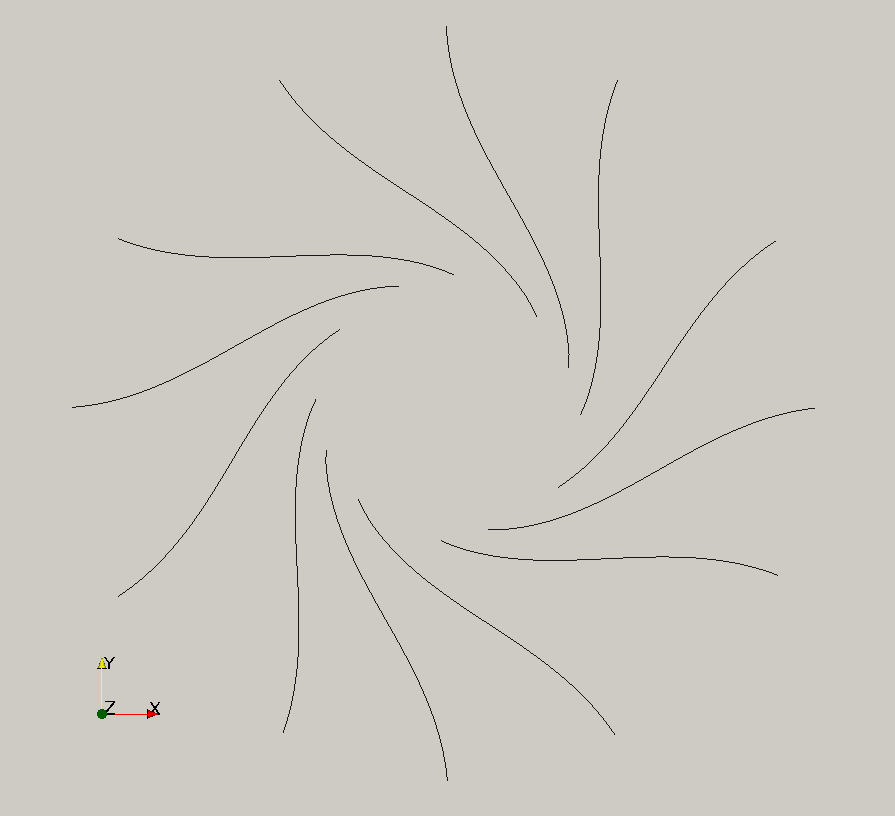
\includegraphics[width=.8\linewidth]{figs/bottom_thermal_only}
 \caption{Horizontal drawings of the curvature functions for the bottom tier
 vanes. The max angle is $85^{\circ}$, or $5^{\circ}$ less than azimuthal.}
 \label{fig:thermal_vane_bottom}  
\end{minipage}\hfill
\begin{minipage}{0.45\textwidth}
\centering
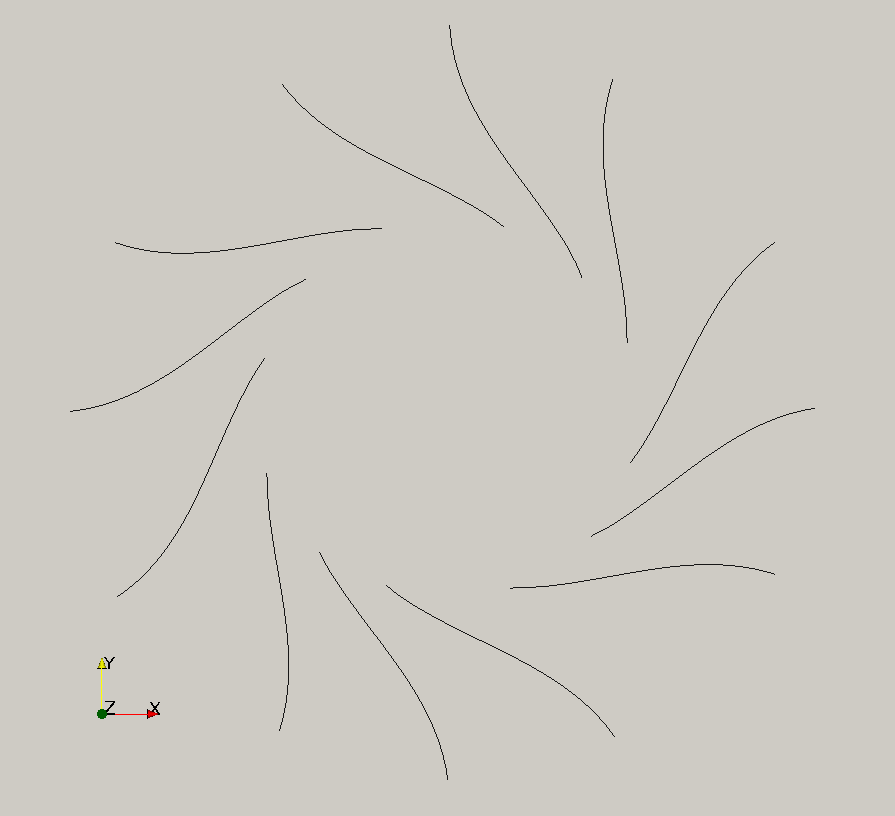
\includegraphics[width =0.8\textwidth]{figs/top_thermal_only}
\caption{Horizontal drawings of the curvature functions for the top tier
 vanes. The max angle is $70^{\circ}$, or $20^{\circ}$ less than
 azimuthal.} 
 \label{fig:thermal_vane_top}  
\end{minipage}
\end{figure}

\begin{figure}[htb]
\centering
\begin{minipage}{0.45\textwidth}
\centering
 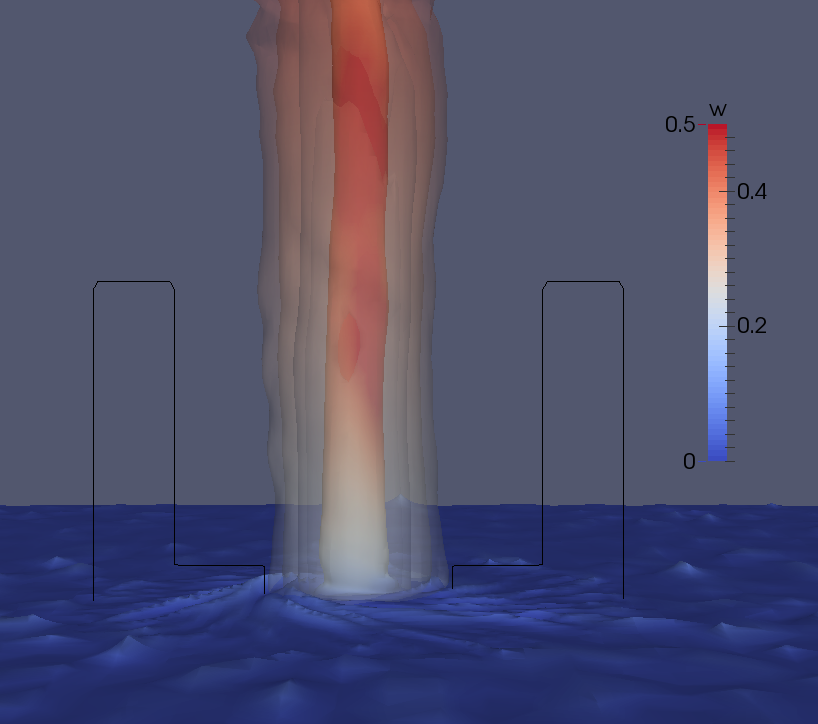
\includegraphics[width=.8\linewidth]{figs/3d}
 \caption{Isocountours of the inner thermal core
  visible through semi-transparent contour around azimuthal velocity,
  colored by vertical velocity. This shows that the thermal core creates
 an upward flow, which entrains and rotations fluid around it. An
 outline of the region of virtual vanes has been drawn.}
 \label{fig:thermal}  
\end{minipage}\hfill
\begin{minipage}{0.45\textwidth}
\centering
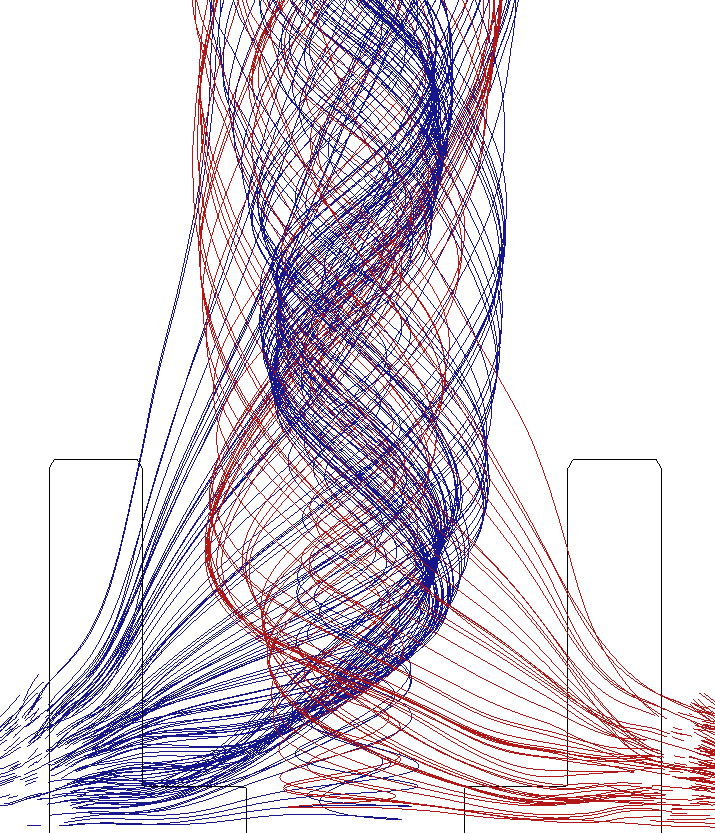
\includegraphics[width =0.8\textwidth]{figs/entrainment}
\caption{Fluid entrainment around the apparatus. This was drawn by
 seeding particles into the averaged flowfield and then advancing them
 using an RK4 time integrator. An outline of the
  virtual vanes are drawn to show the region of forcing.}
 \label{fig:entrain}  
\end{minipage}
\end{figure}


% \begin{figure}[htb]

%  \begin{subfigure}{.55\textwidth}
%   \centering
%   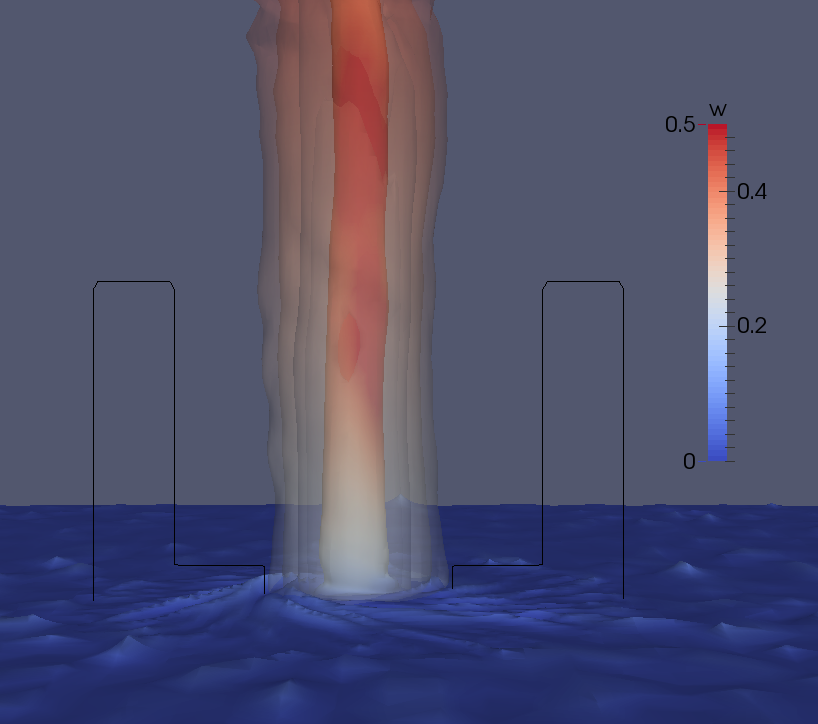
\includegraphics[width =0.7\textwidth]{figs/3d}
%   \caption{Isocountours of the inner thermal core
%   visible through semi-transparent contour around azimuthal velocity,
%   colored by vertical velocity. An outline of the region of virtual
%   vanes has been drawn.}
%   \label{fig:thermal}  
%  \end{subfigure}%
%  \begin{subfigure}{.4\textwidth}
%   \centering
%   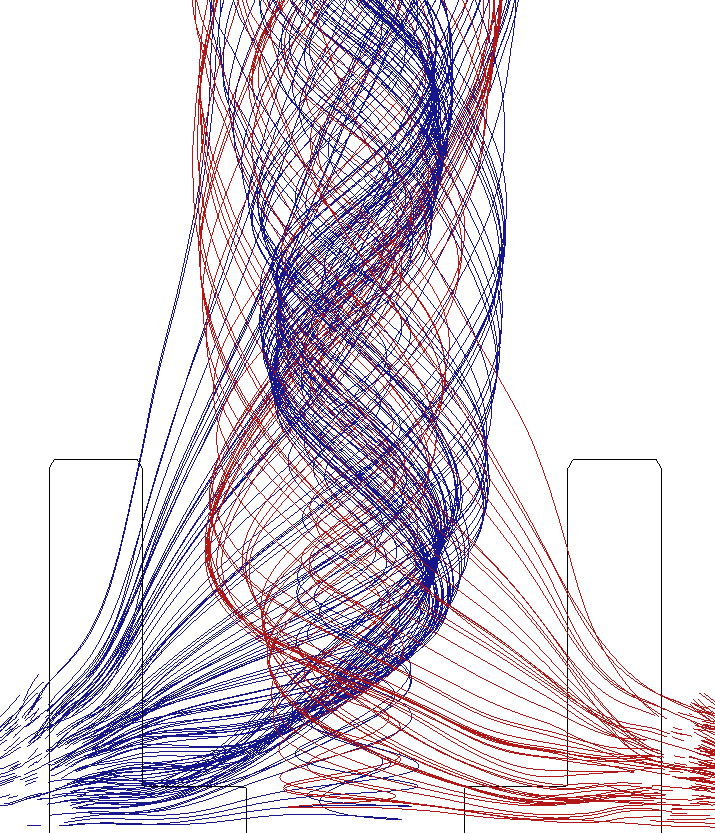
\includegraphics[width =0.8\textwidth]{figs/entrainment}%
%   \caption{Fluid entrainment around the apparatus. An outline of the
%   virtual vanes are drawn to show the region of forcing.} 
%   \label{fig:entrain}  
%  \end{subfigure}%
% \end{figure}

The results shown were from transient solutions (the unsteady virtual
vanes) and so the images of the fields are averages of fifty snapshots
of the solution taken over the course of ten minutes. In general, the
averaging times are selected to be approximately 20 to 30 wash-out
times, where a wash-out is defined as the time required for a particle
at the base of the apparatus to flow out through the top boundary. The
kinetic energy flux through the top of the vanes for this case is about
53 watts. The solution demonstrates several features characteristic of
naturally occurring dust devils. Figure~\ref{fig:thermal} shows a
temperature isocontour set at threshold of 3 Celsius higher than the
ambient fluid temperature. This value was selected because it was noted
by Sinclair~\cite{Sinclair1969} as characteristic of the thermal core 
temperature above the ambient temperature observed in dust devils. The
image depicts a tight, coherent thermal plume roughly the same size as
the inner diameter of the lower vanes. As anticipated, this hot flow is
acting like a chimney, generating a large vertical velocity which in
turn entrains air from the outside.  

An image of the entrainment is shown in Figure~\ref{fig:entrain}. The
image was created by tracking particles as they convect through the
device. Tracer particles were seeded into the averaged flowfield and
then advancing through the field using a fourth order Runge-Kutta integrator.  
There is clearly a tight inner vortex with significant azimuthal
velocity and a broader region of entraining fluid through the upper tier
of vanes. This is consistent with the imagined structure of a dust devil
presented in Figure~\ref{fig:cartoon}.    

\begin{figure}[htb]

 \centering
 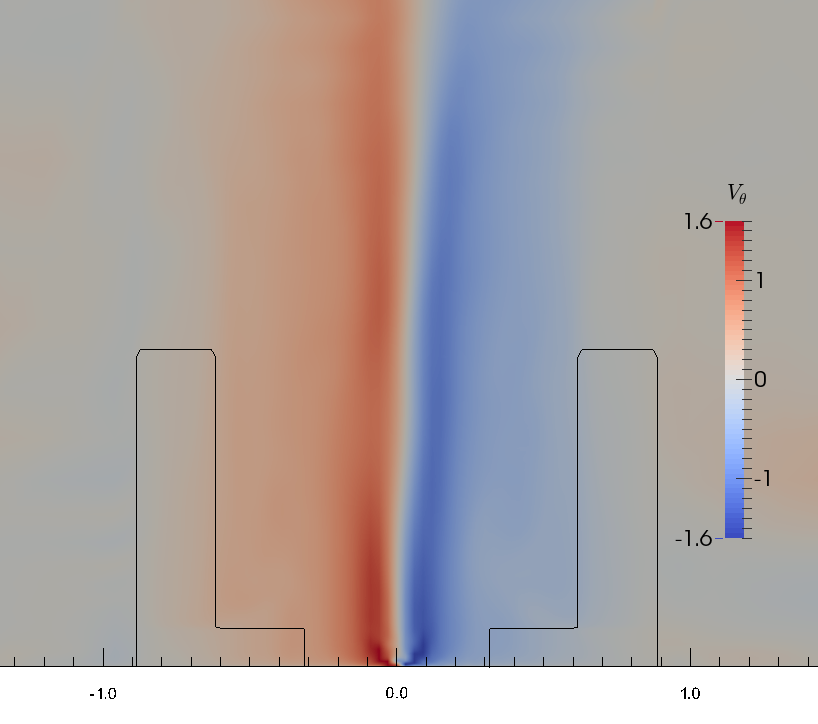
\includegraphics[width=.4\linewidth]{figs/vt}
 % \caption{Azimuthal Velocity}
 % \label{fig:vt-to}
 \hfill
  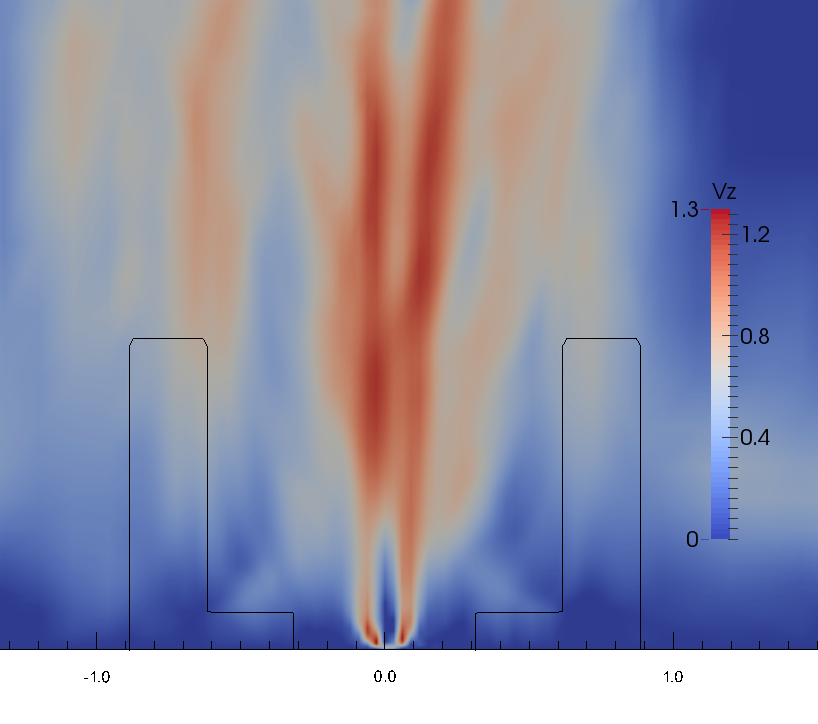
\includegraphics[width=.4\linewidth]{figs/vz}
 %\caption{Vertical Velocity}
 % \label{fig:vz-to}
 \\
  \centering
  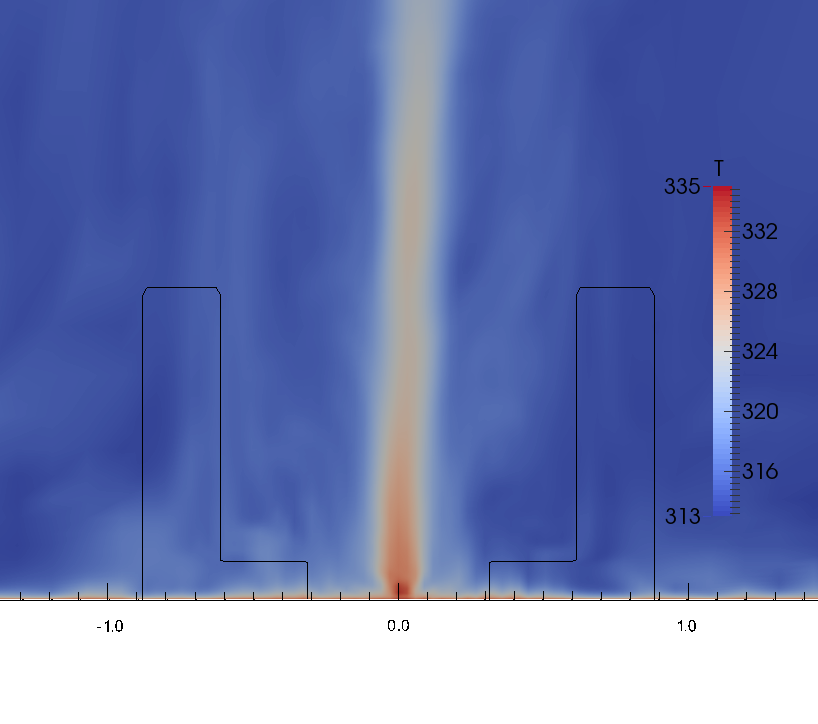
\includegraphics[width=.4\linewidth]{figs/t}
 %\caption{Temperature}
 % \label{fig:t-to}
 \hfill
 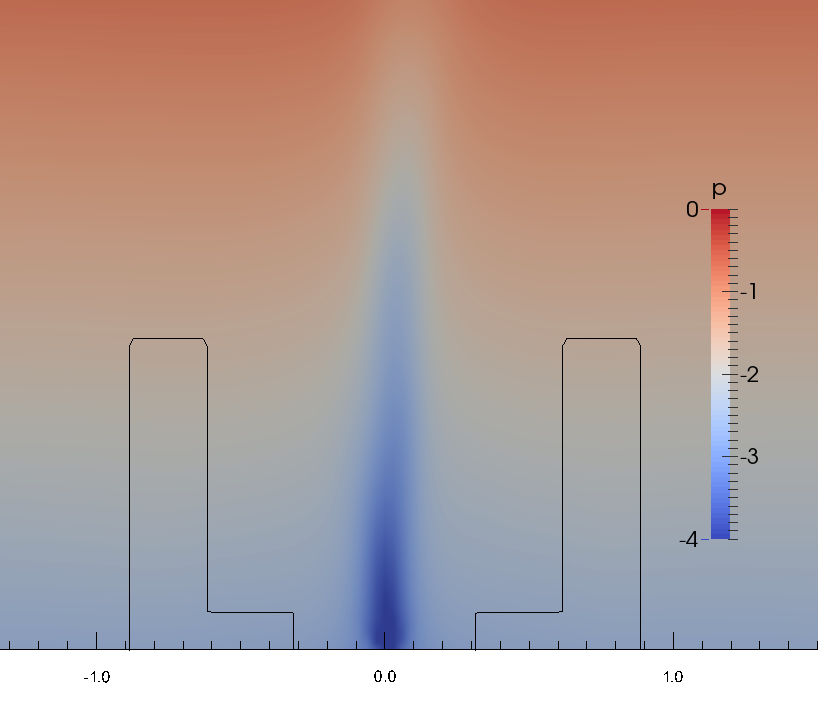
\includegraphics[width=.4\linewidth]{figs/p}
 % \caption{Pressure}
 % \label{fig:p-to}
 \caption{Time averaged vertical slices through the center of the device
 for the thermal-only cases. Black lines indicate the location of the
 vanes. The top left is the azimuthal velocity (v), and the top right
 the vertical velocity, w. The bottom row shows the same plane, but now for the
 temperature and pressure.} 
 \label{fig:to-vert}
\end{figure}

%
%
%
Figure~\ref{fig:to-vert} depicts several vertical slices through the SoV
for various state variables. A strong thermal plume is visible at the
center of the device, which drives a vertical velocity. The fluid flow
is entrained by this vertical movement and pulled radially into the
center while being turned by the turning vanes. Notice also the low
pressure ``eye'' at the center of the flow, and the modest downward flow
in the center of the vertical velocity, consistent with
Figure~\ref{fig:cartoon}. 

\begin{figure}[htb]

 \centering
  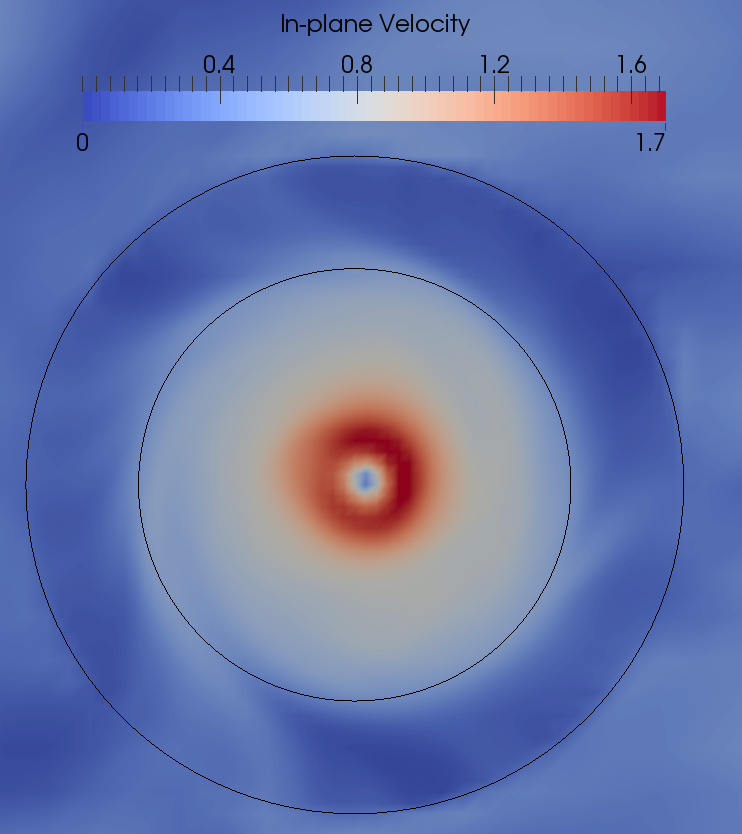
\includegraphics[width=.32\linewidth]{figs/vt_hor}
 %\caption{Azimuthal Velocity}
 % \label{fig:vt-to}
 \hfill
  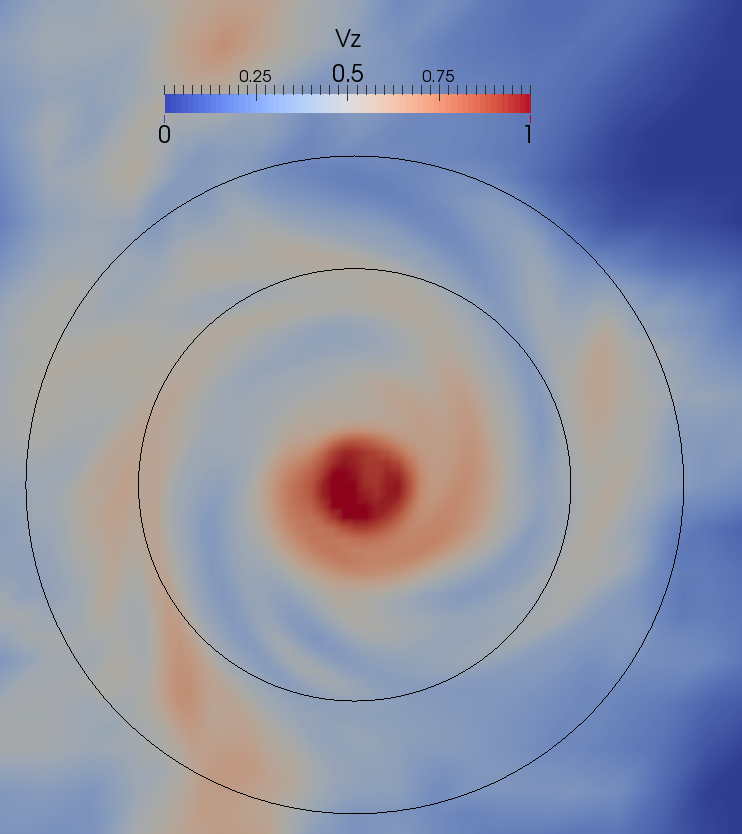
\includegraphics[width=.32\linewidth]{figs/vz_hor}
 % \caption{Vertical Velocity}
 % \label{fig:vz-to}
 \hfill
  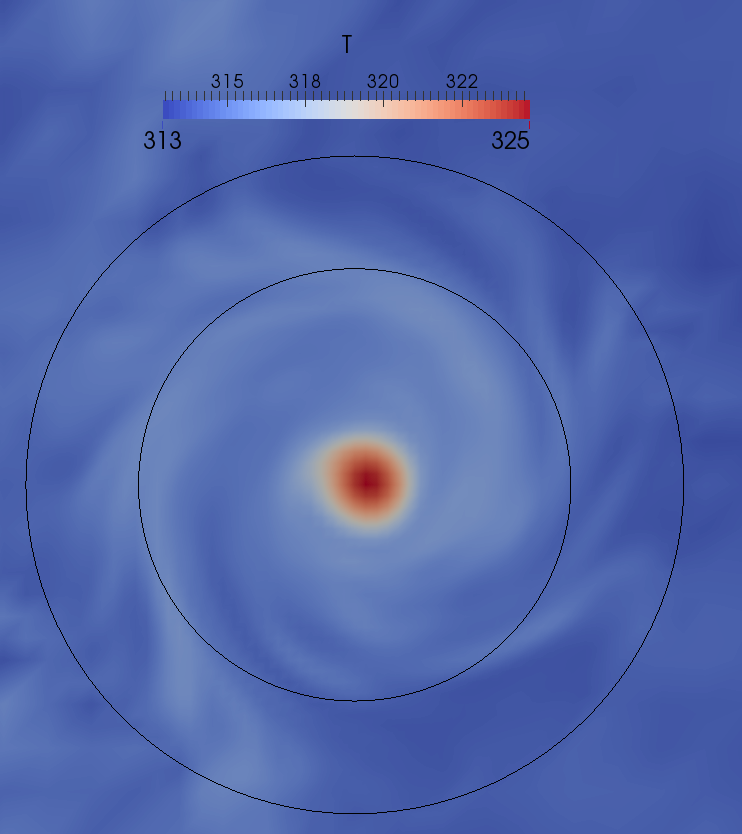
\includegraphics[width=.32\linewidth]{figs/t_hor}
 % \caption{Temperature}
 % \label{fig:t-to}
 \caption{Time averaged horizontal slices taken at the height of the
 second tier of vanes for the thermal-only cases. The left most image
 depicts the in-plane velocity. The middle image the vertical velocity,
 and the image on the right the temperature field. These images show a
 clear thermal plume driving a strong vertical velocity. Notice also the
 low downward velocity ``eye of the storm'' in the first image. In
 contrast to the wind cases, the vortex is well-anchored in the center
 of the apparatus. An outline of the virtual vanes are drawn to show the
 region of forcing.}
 \label{fig:to-hor}
\end{figure}

Figure~\ref{fig:to-hor}, depicts several horizontal slices
through the SoV for the same state variables. It can be seen that the
large velocities are highly localized to a region just inside the
vanes. Likewise, the entrainment of fluid is limited to a region
immediately surrounding the vanes.\todo{fix axes to make readable} 
%
% conclusion of thermal only
%
Finally, the thermal plume is relatively narrow compared to the diameter
of the device. It is desirable to broaden the thermal plume, as this
would create a larger vertical momentum flux and consequentally a larger
kinetic energy flux.\todo{kill?}  

The diameter of the thermal core is therefore a critical flow
characteristic in the thermal-only conditions. However, a means of
setting the thermal plume's thickness is not presently 
known. Regardless, these slices lend credibilty to the 
notion that our turning vane configuration is generating something with
visible parallels to a naturally occurring dust devil.   

\section{Wind}

The wind case is for a 5 m/s ambient wind with a ground temperature of
335 Kelvin and freestream temperature of 313 Kelvin. There is no ambient
velocity and the boundary conditions are as described in
Chapter~\ref{sec:bc}. The vanes are drawn in
Figures~\ref{fig:wind_bottom} and \ref{fig:wind_top}. These images show
the straight vane case, and a cone that sits on top of the second tier of vanes. 
As in the previous section, these images are representative
curves of the body forcing field, and do not actually represent vane
surfaces. The vanes are represented as in Chapter~\ref{subsec:vane}. 
These images are created by tracing the path a particle follows through
the forcing field. The region of forcing is between $\{0.96-3.4\}$ meters
for the bottom tier, and $\{1.5-3.4\}$ meters for the top tier. Overall,
the system is three meters tall, with the short first tier only standing
0.3 meters high. The top and bottom tiers have final angles of
$70^{\circ}$ and $80^{\circ}$, respectively.\todo{add newer and fixed up
wind images}

\begin{figure}[htb]
\centering
\begin{minipage}{0.45\textwidth}
\centering
 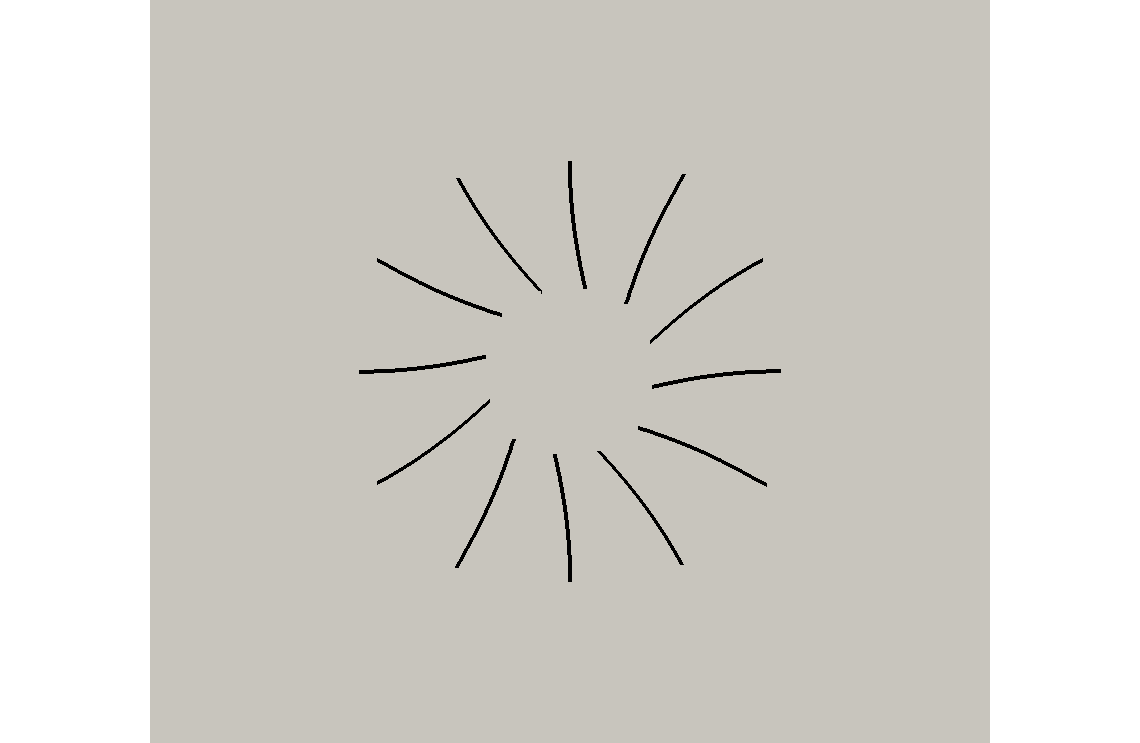
\includegraphics[width=.8\linewidth]{figs/wind_bottom}
 \caption{Horizontal drawings of the bottom tier vanes. These are curved 
 vanes with a final angle of $80^{\circ}$.}
 \label{fig:wind_bottom}  
\end{minipage}\hfill
\begin{minipage}{0.45\textwidth}
\centering
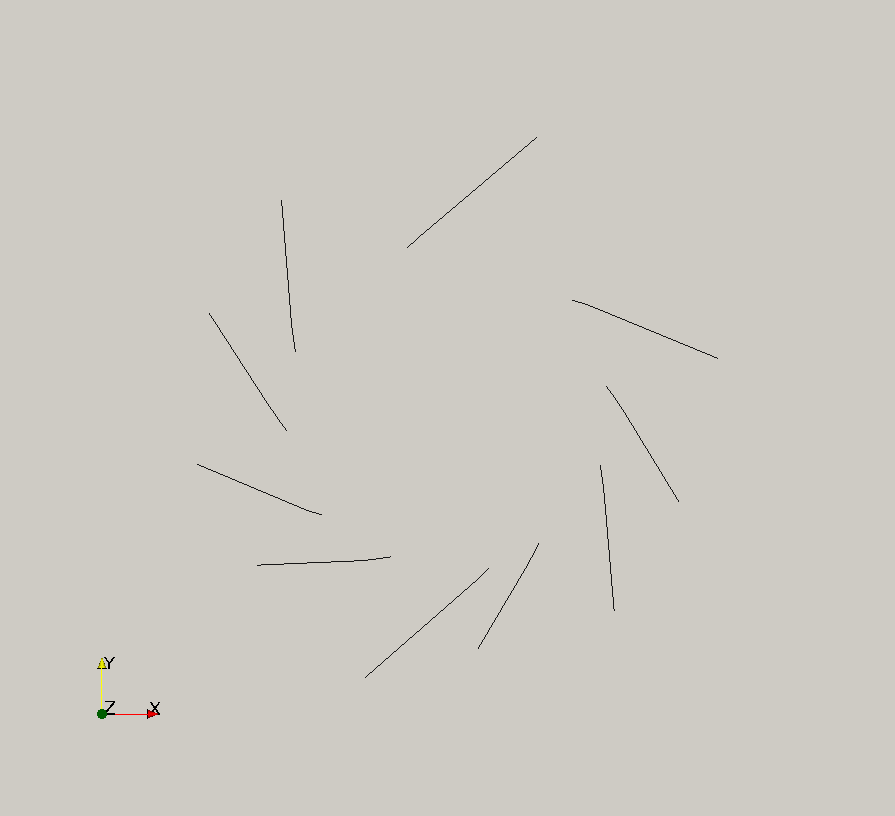
\includegraphics[width =0.8\textwidth]{figs/wind_top}
\caption{Horizontal drawings of the top tier vanes. These are straight
 angle vanes set at $70^{\circ}$.} 
 \label{fig:wind_top}  
\end{minipage}
\end{figure}


%
% horizontal slices
%
\begin{figure}[htb]

  \centering
  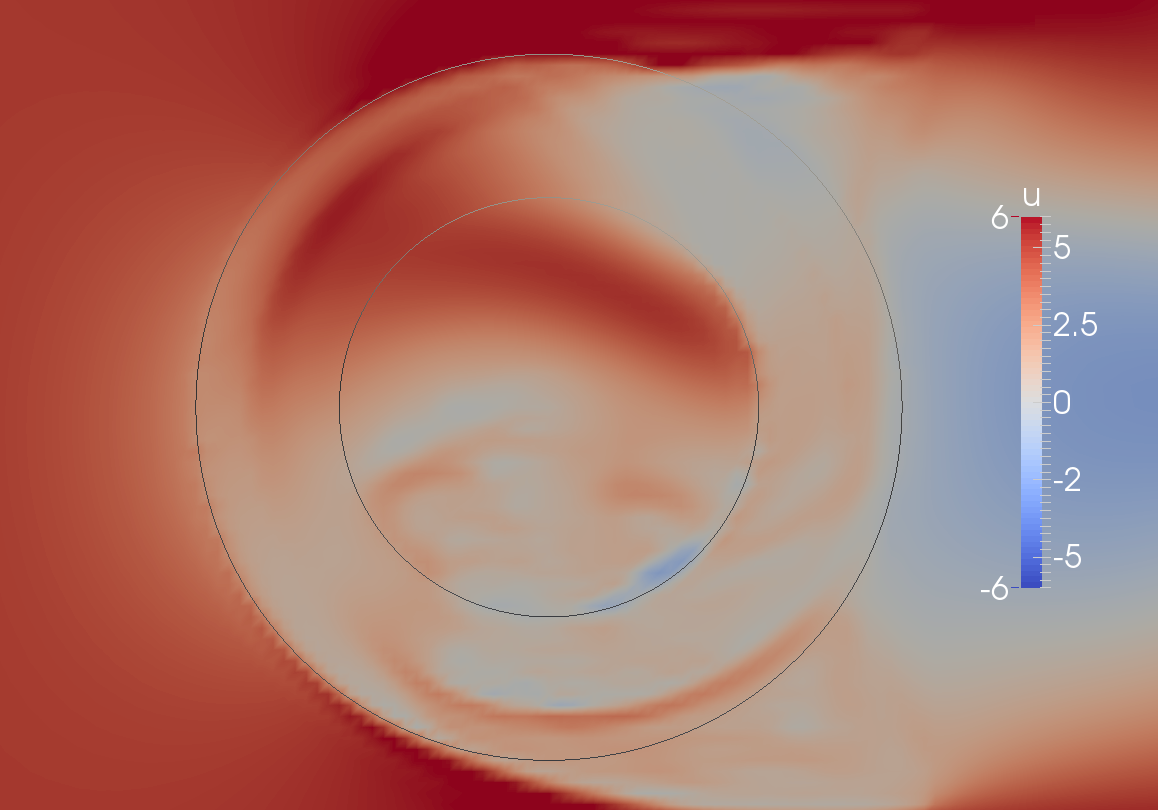
\includegraphics[width=.47\linewidth]{figs/wind_u}
 %\caption{Streamwise}
 % \label{fig:vt-wind}
 \hfill
  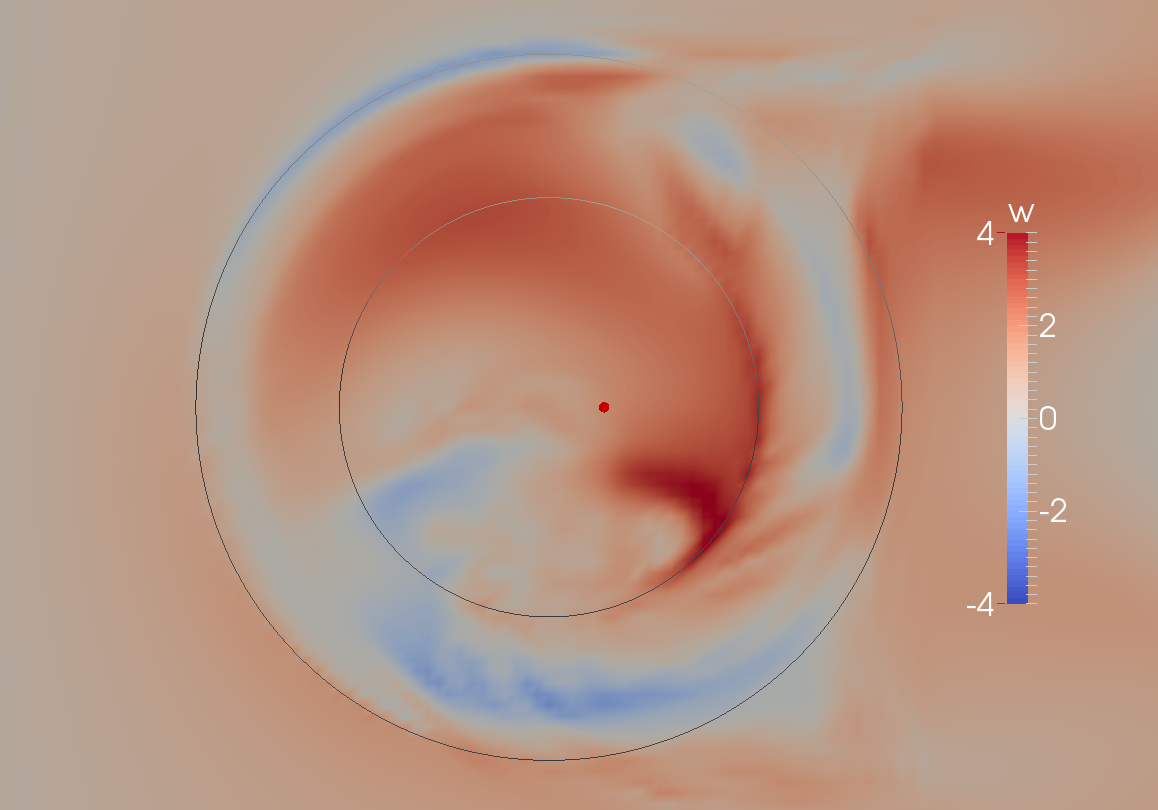
\includegraphics[width=.47\linewidth]{figs/wind_w}
 %\caption{Vertical Velocity}
 % \label{fig:vz-wind}
 \\
  \centering
  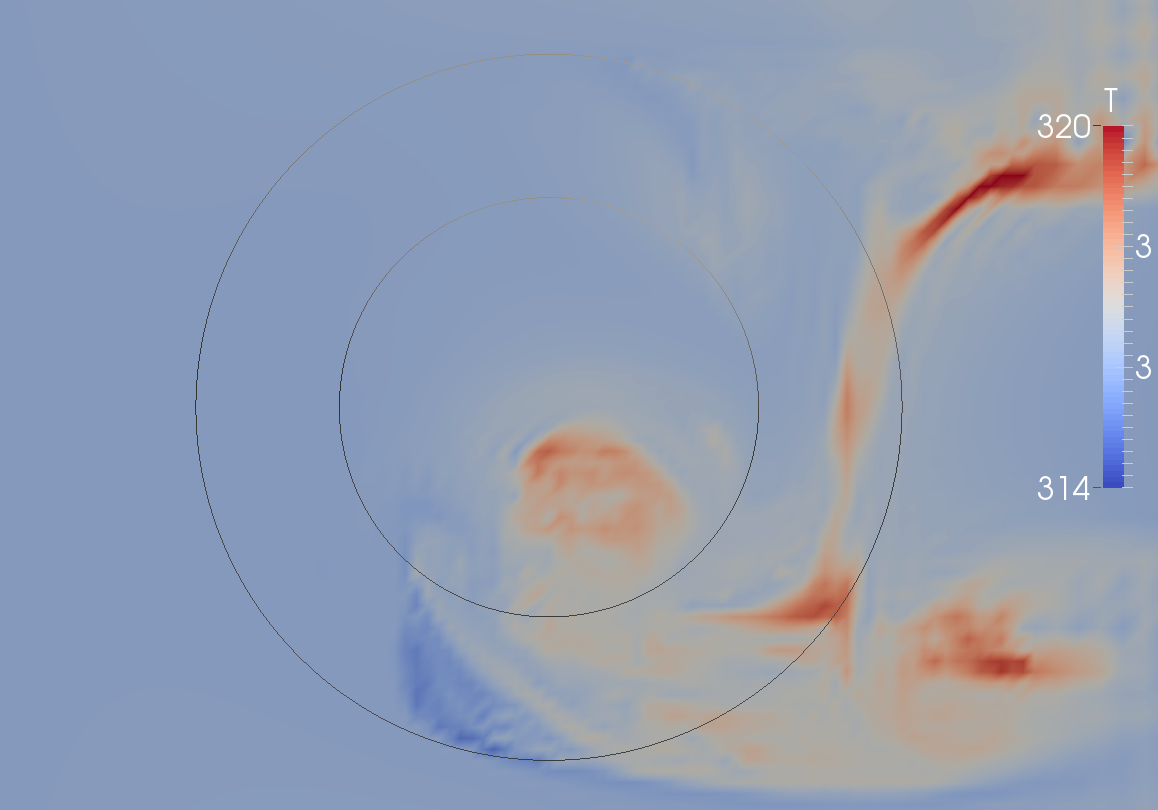
\includegraphics[width=.47\linewidth]{figs/wind_t}
 \hfill
  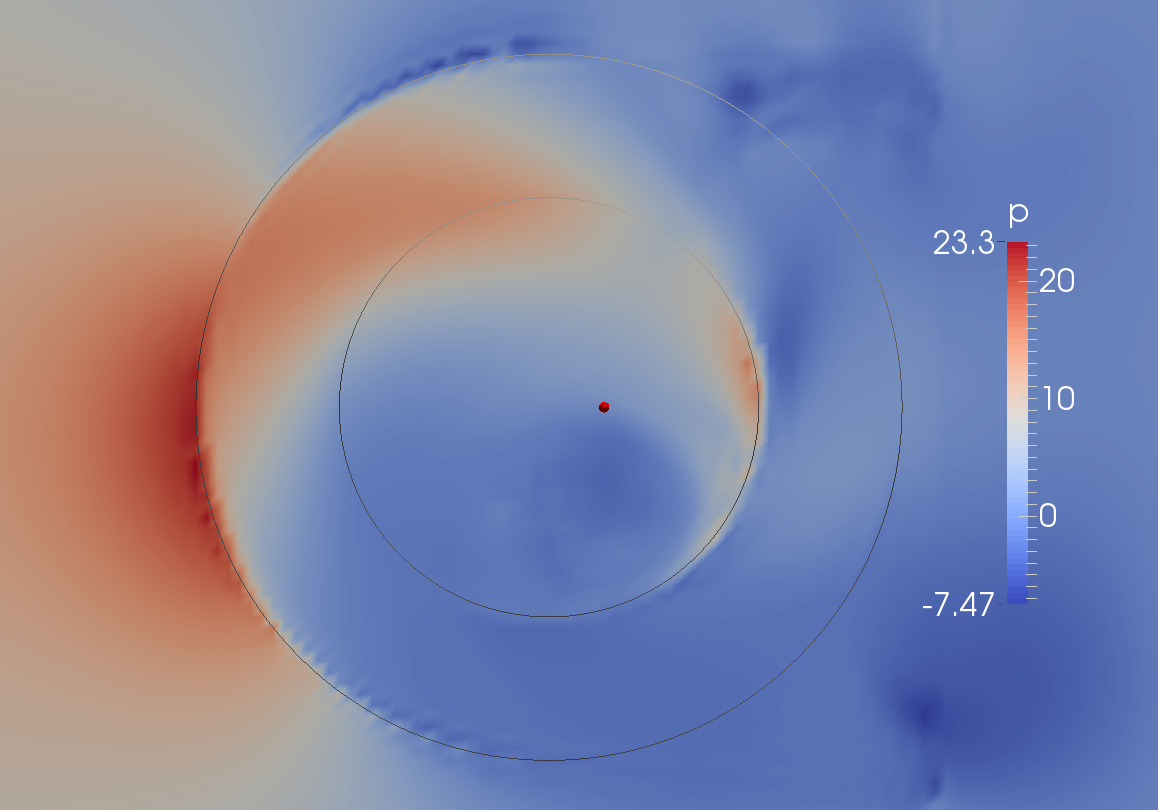
\includegraphics[width=.47\linewidth]{figs/wind_p}
  %\label{fig:p-wind}
 \caption{Time averaged horizontal slices taken at the height of the
 vanes for the wind cases. The streamwise velocity shows a large
 penetration in the region where the vanes are not blocking, and in the
 other regions the flow is blocked and flows around. The vertical
 velocity is disorganized and does not show the ``two cell'' structure
 as in the thermal-only cases.  Note that an off-center thermal plume is
 visible, as well. An outline of the virtual vanes are drawn to show the
 region of forcing.}  
 \label{fig:wind-hor}
\end{figure}


Horizontal slices of the azimuthal and vertical velocities, and the 
temperature and pressure fields are shown in
Figure~\ref{fig:vz-wind-vert}\todo{bring me back}. The freestream
velocity is traveling from left to right at 5 m/s\todo{is 5 right?}, which was set based
on ambient velocity measurements made by the experimental team from the
field. While the structure is undoubtedly different than the
thermal-only cases shown previously, we can nevertheless see that a
thermal plume is forming along with a rotating velocity structure. In
general the wind cases are more disorganized, with less obviously
visible coherent structure. Notice however that the magnitude of
velocities are several times larger than in the thermal-only cases, and
the kinetic energy flux through the vanes is also significantly higher.   

%
% vertical
%

\begin{figure}[htb]
  \centering
  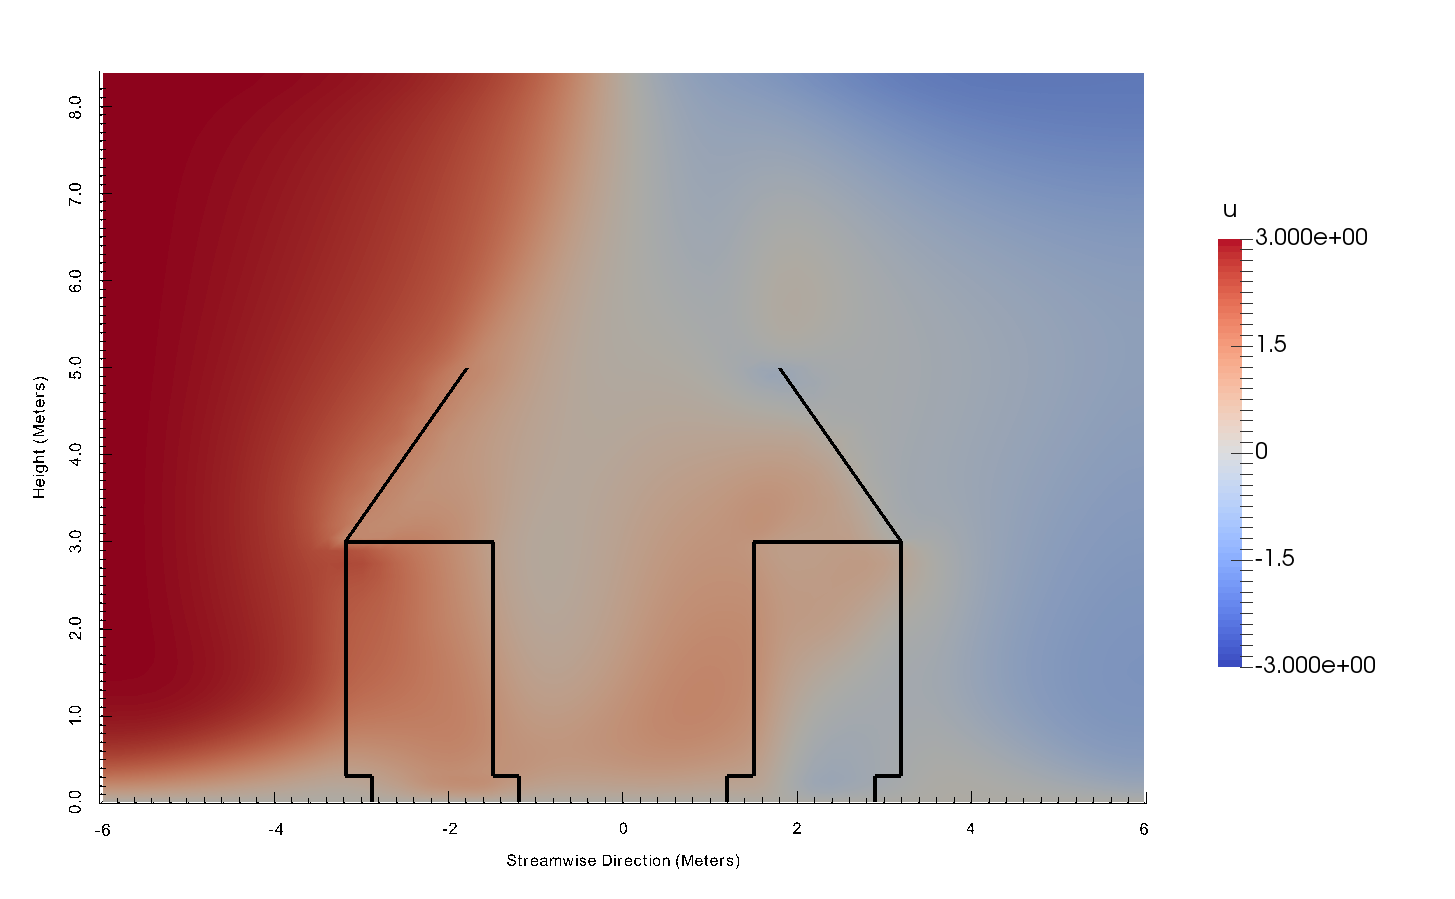
\includegraphics[width=.45\linewidth]{figs/wind_u_vertical}
  \hfill
  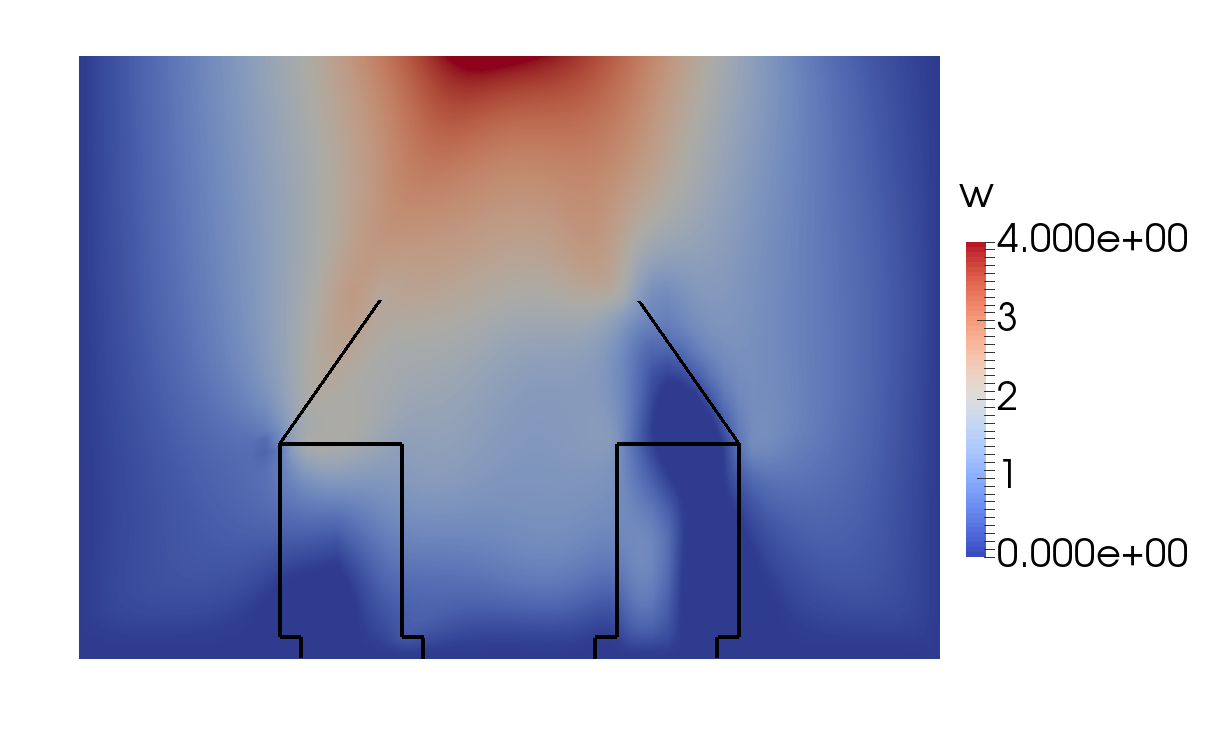
\includegraphics[width=.45\linewidth]{figs/wind_w_vertical}
  \\
  \centering
  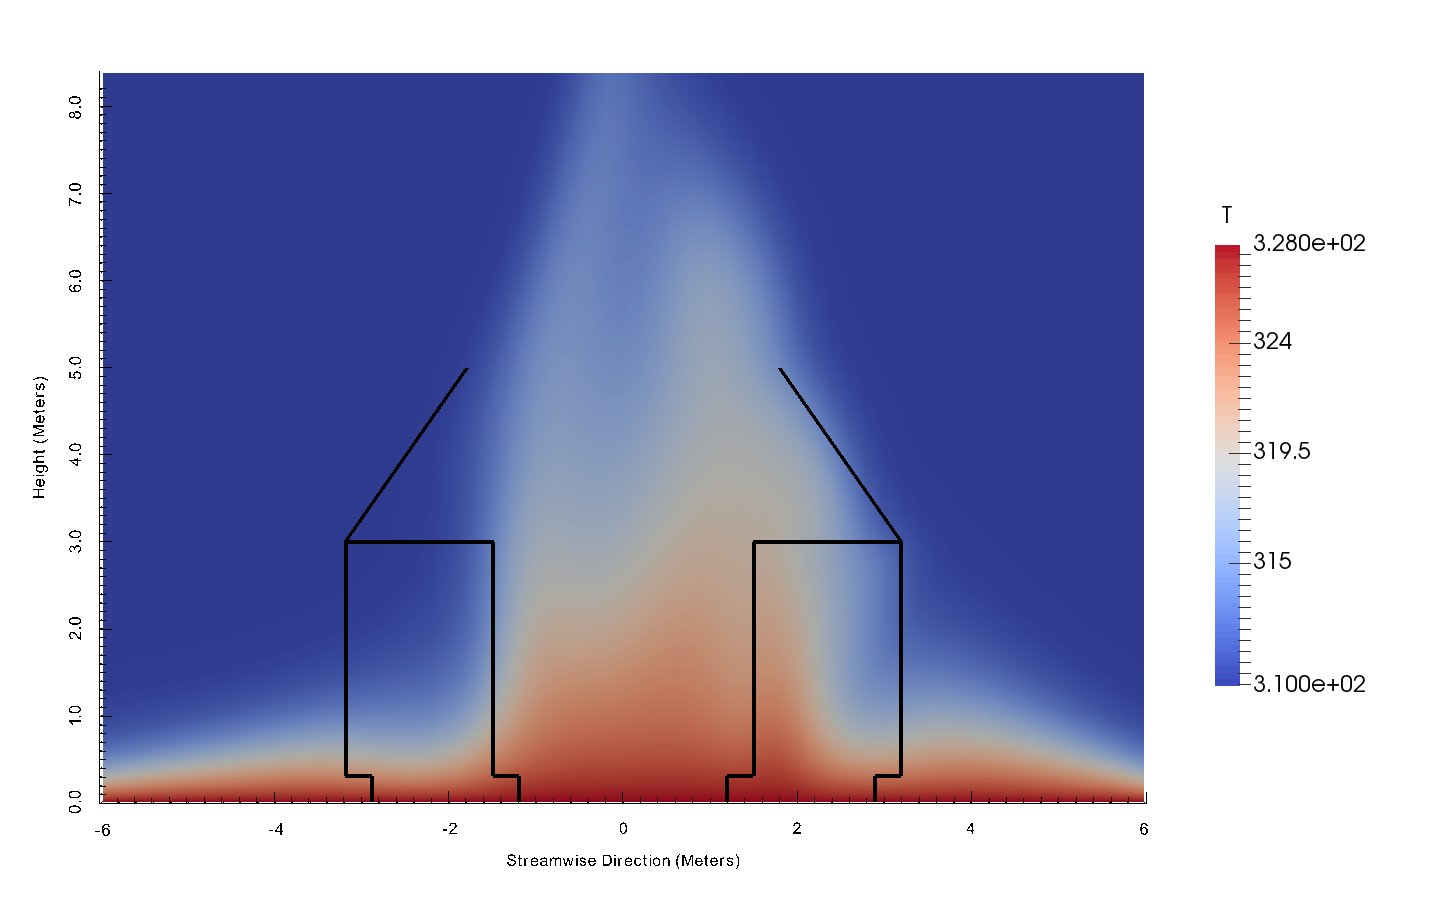
\includegraphics[width=.45\linewidth]{figs/wind_t_vertical}
  \hfill
  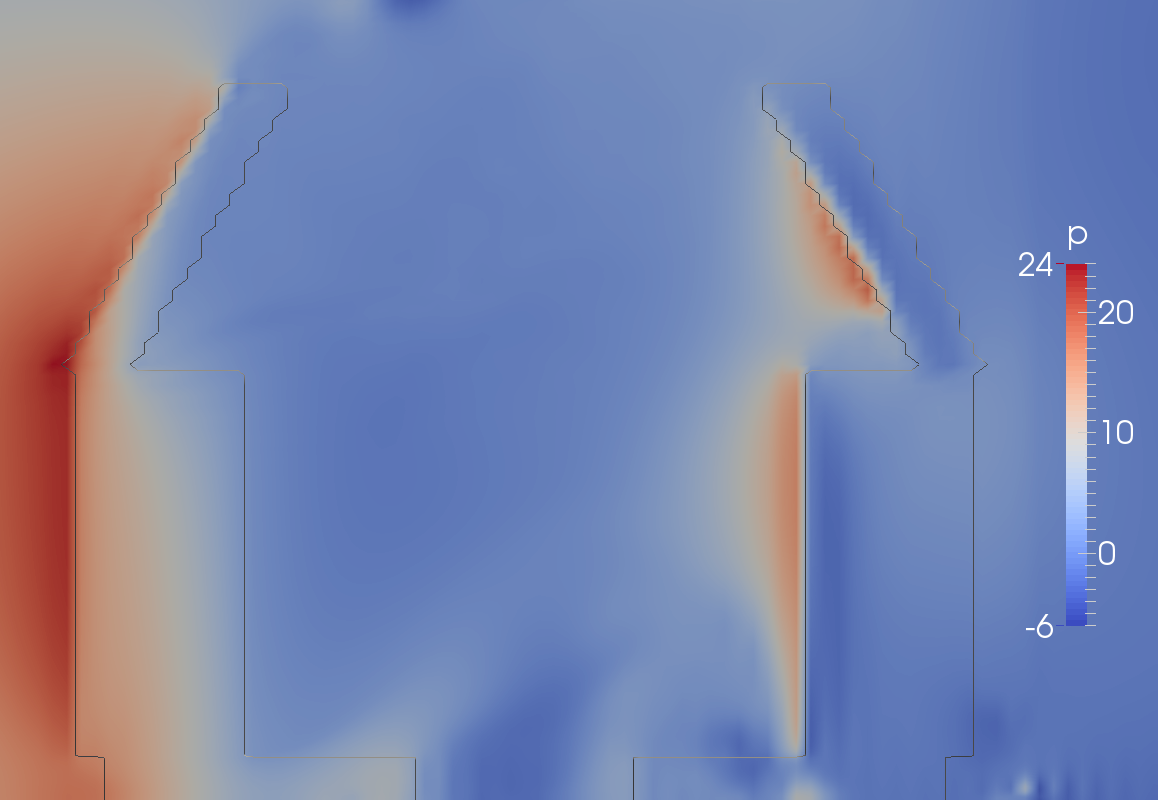
\includegraphics[width=.45\linewidth]{figs/wind_p_vertical}
  \\
 \caption{Time averaged vertical slices from the center of the device
 for the wind cases. A great deal of flow is radially entrained by the
 first tier of vanes, consistent with the approach proposed in
 Figure~\ref{fig:cartoon_vanes}. Notice that while the temperature field
  appears to be quite modest, this is due to the fact that the thermal
  column is not well centered. The full column is visible in
  Figure~\ref{fig:field_real}.}
 \label{fig:wind-ver}
\end{figure}

The vertical slices are shown in Figure~\ref{fig:wind-ver}. In this
case, the lower tier of vanes are where the majority of flow is 
entering the center of the apparatus, while the second tier of vanes are
blocking the ambient wind and providing protection for the vortex column. 

The thermal plume is significantly less
visible than in the thermal-only cases. While the
thermal-plume is necessarily weaker relative to the wind, some of this
is also due to the plume no longer being directly centered in the
flow. The plume is more visible using isocountors to render a
three-dimensional surface. 
To visualize the difference between the vertically varying ambient
temperature and the warmer thermal plume, we use the potential
temperature, defined as,\todo{kill this?} 
\begin{equation}
  \tau(x,y,z) = T(x,y,z) -T_{\text{in}}(z) 
   \label{eqn:tau}
\end{equation}
where $T_{\text{in}}$ is the inflow temperature, described
in Chapter \ref{sec:bc}. In this way the background potential
temperature is nearly zero, and larger values represent deviations from
the base flow temperature. The isocountour of a three Kelvin is 
shown in Figure~\ref{fig:field_real}. This value was selected as
it was noted as sufficient for formation of a dust devil by
Sinclair~\cite{Sinclair1969}. It is clear from the image that a 
strong thermal column does exist even in the 5 m/s wind cases. 

%
% tiso
%
  \begin{figure}[!htb]
   \begin{center}
    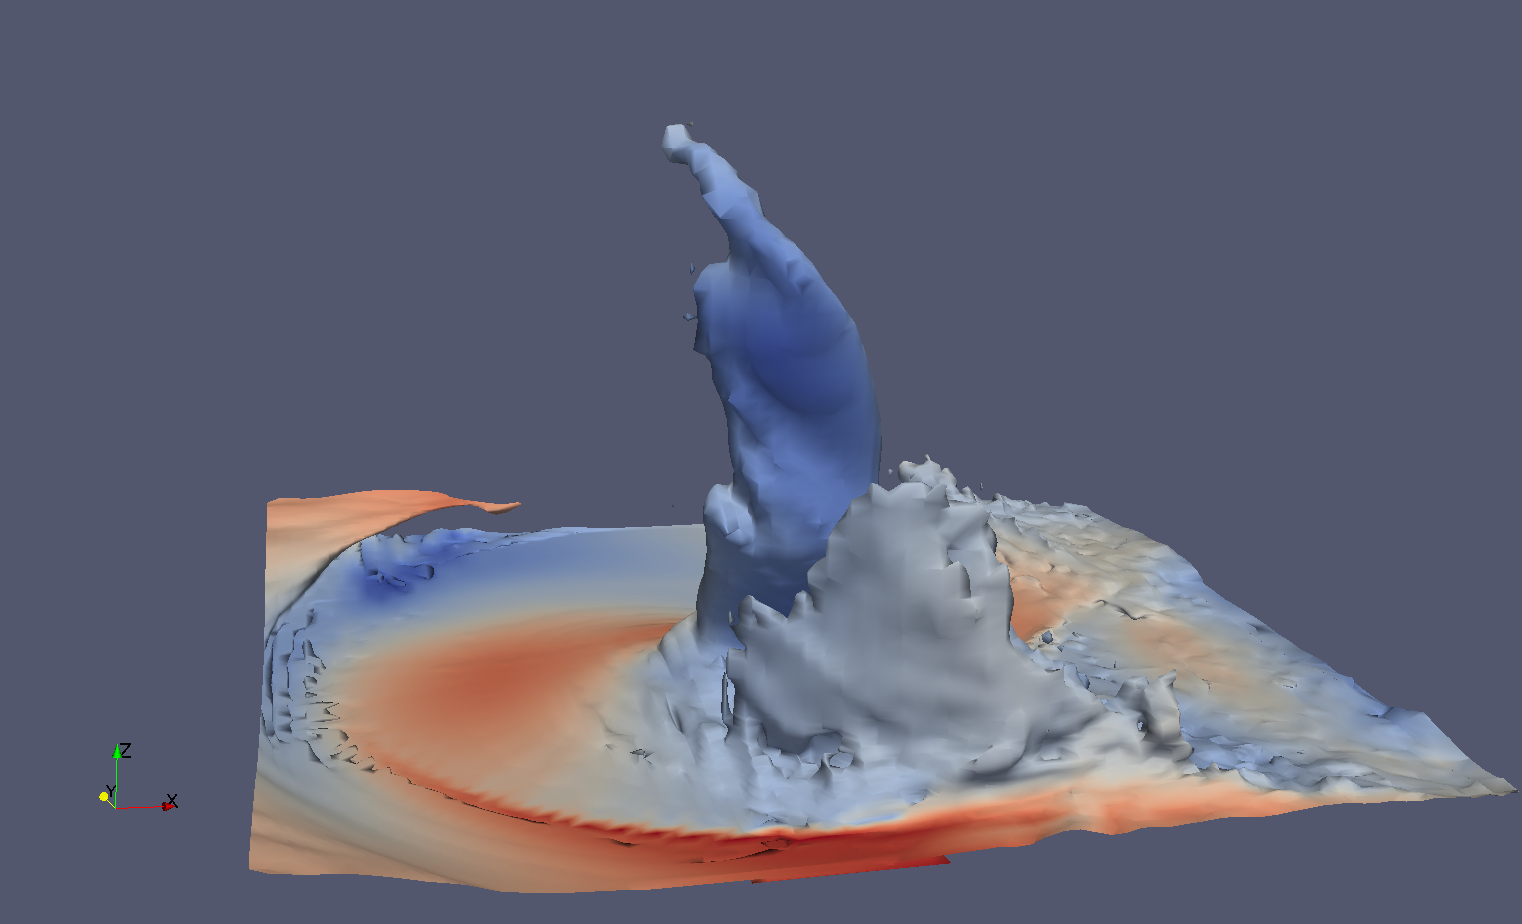
\includegraphics[width = 12 cm]{figs/t_iso}
    \caption{Iso-contour of the thermal plume. Here, the isocontour is
    labelled by the potential temperature, $\tau$, as defined in
    Equation \ref{eqn:tau}. A strong thermal column has visibly formed. The
    figure is colored by the streamwise velocity, and shows the thermal
    column also has rotation.} 
    \label{fig:field_real}
   \end{center}
  \end{figure}

\section{Optimization}

In this section results from a representative optimization
in a thermal-only case are discussed, to demonstrate the optimization 
process employed so far. This is a typical mode of scientific and
engineering inquiry, where a hypothesis regarding system operation is
developed, followed by testing of the hypothesis, and further
iterations.  

This series of simulations are all runs with different system
configurations conducted in a common ambient scenario, that of the
unsteady thermal-only simulations described in Chapter~\ref{sec:bc}. 

Our objective is to maximize the energy that can be 
extracted from the synthetic dust devil. As a surrogate to this
quantity, consider the kinetic energy flux through a horizontal plane
near the top of the vanes, where a turbine will ultimately be
placed. This is a surface integral~\cite{landau1959fm},

% flow.io is awesome
% https://support.draw.io/questions/2949135/how-to-use-mathematical-typesetting
%
%
%https://www.draw.io/?url=https%3A%2F%2Fjgraph.github.io%2Fdrawio-diagrams%2Fdiagrams%2Fmath.xml
%


%% \begin{equation}
%%  \dot E = -\oint \rho \textbf{v}(\frac{1}{2}v^2 + e) \cdot d \textbf{f}
%% \end{equation}
%% where $e$ is the internal energy. % and $d\textbf{f}$ the. 
%% For our problem, we consider an incompressible fluid flowing through a
%% flat horizontal region interior to the vanes in the x-y plane, which
%% results in, 

 \begin{equation}
  \dot{ \text{KE}} = -\frac{\rho }{2} \int V_z (V_{\theta}^2 + V_z^2 ) dA.
 \end{equation}

\begin{figure}[htb]
 \centering
 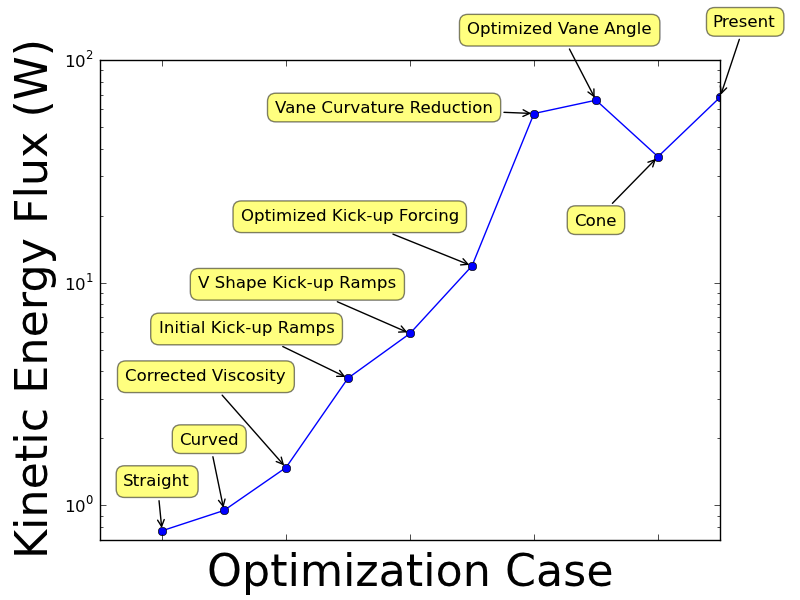
\includegraphics[width=.75\linewidth]{figs/opt_plot}
 \caption{This plot diagrams the improvements to the calculated flux for  
 each iteration of system configuration in the thermal-only optimization
 effort. Every iteration is labeled by design change. This list
 only highlights the accepted improvements, and the numerous runs of a
 particular parameter configuration that yielded inferior power output
 are not shown. }
 \label{fig:opt_plot}
\end{figure}


% \begin{figure}[htb!]
%  \begin{subfigure}{.5\textwidth}
%   \centering
%   
\includegraphics[width=.75\linewidth]{figs/before_vanes}
%   \caption{Vanes before optimization}
%  \end{subfigure}%
%  \begin{subfigure}{.5\textwidth}
%   \centering
%   
\includegraphics[width=.8\linewidth]{figs/after_vanes}
%   \caption{Vanes after optimization}
%  \end{subfigure}%
%   \caption{Can we do this}
%  \label{fig:vt-wind-vert}
% \end{figure}\todo{need better figure}




\begin{figure}[htb]
  \centering
 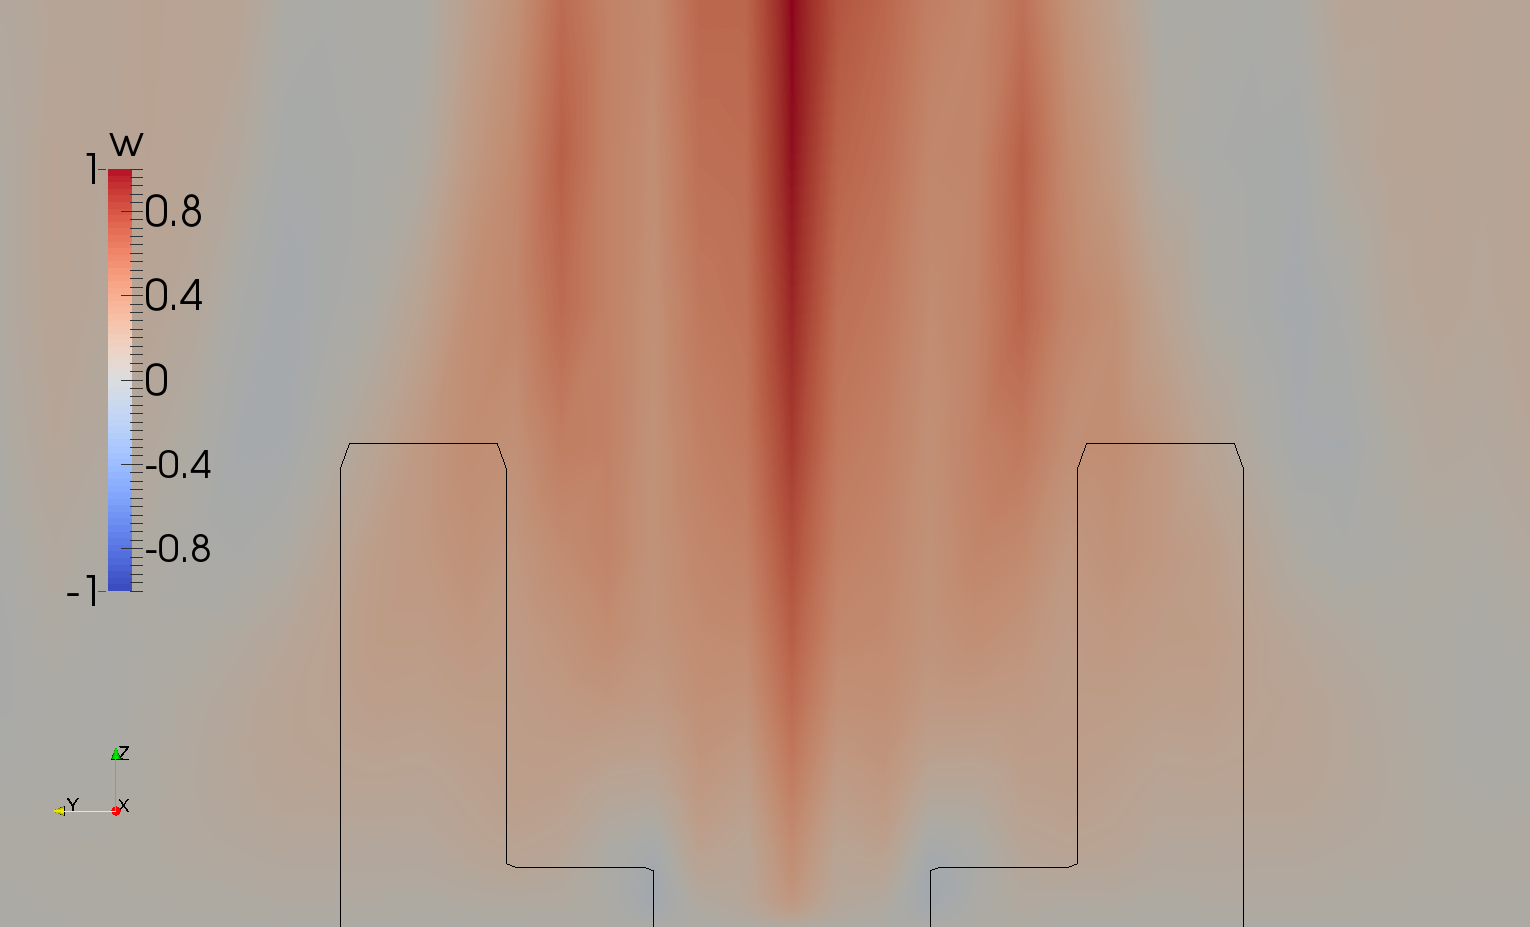
\includegraphics[width=.45\linewidth]{figs/before_opt}
 \hfill
 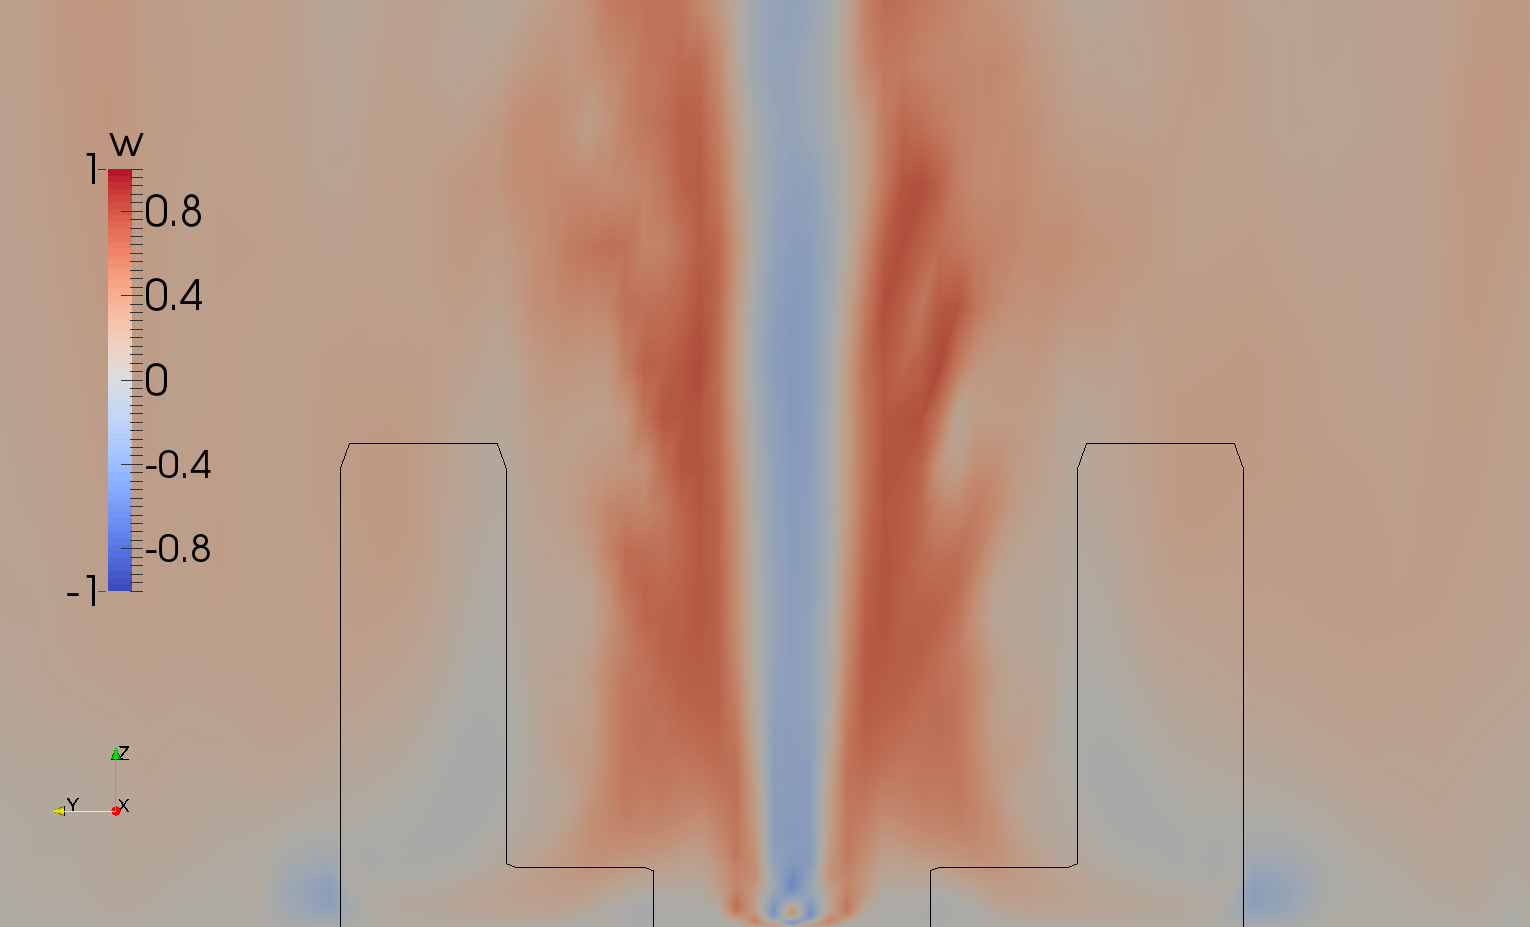
\includegraphics[width=.45\linewidth]{figs/after_opt} \\
  \caption{These are vertical slices taken at the center of the vanes of
 the vertical velocity taken before and after the numerous optimizations
 of the turning vanes detailed in Figure \ref{fig:opt_plot}. In the
 original (left image), the flow produces a narrow plume. In the second
 (right figure), the flow shows stronger vertical velocities in a much
 larger and more organized vortex. The flow has also transitioned into a
 ``two-cell'' structure akin to that observed in the naturally occuring
 phenomena as discussed in Chapter \ref{subsec:phenomena}. An outline of
 the virtual vanes are drawn in black to show the region of forcing.}
  \label{fig:opt_flow}
\end{figure}


Using the kinetic energy flux as an objective, the vane geometry has
been optimized. Over approximately tens of iterations, we have
increased the kinetic energy flux by a factor of 88 relative to the
baseline. 

\begin{figure}[htb]
 \centering
 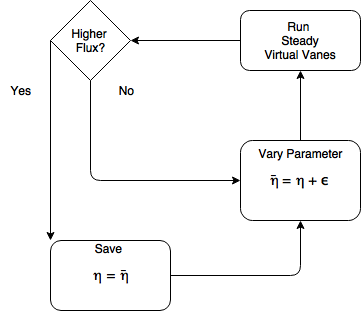
\includegraphics[width=0.75\linewidth]{figs/optimization_flow}
 \caption{A flowchart detailing the optimization heuristic. $\eta$ is
 representative of any SoV geometric parameter, such as the vane angles,
 vane height, cone contraction, etc. $\epsilon$ is a small perturbation
 to the base state, which is not randomly selected but typically is a
 small fraction of the base value. }
 \label{fig:opt_image}
\end{figure}


%Results of several of these iterations are documented in
%Figure \ref{fig:opt_plot}. 
Major adjustments to design in the the vane
shape and angles were made to obtain this improvement. Before and after
images are shown in Figure~\ref{fig:vt-wind-vert}. During this
optimization the 
qualitative character of the solution changed substantially, changing
from a mild upward flow with little rotation to a strongly organized
vortex with a downward central flow and strong azimuthal
velocities. Before and after vertical slices are shown in
Figure~\ref{fig:opt_flow}. Nevertheless, with a peak energy flux for the
final iteration of less than one hundred Watts, significant further 
optimization is necessary for this system to be viable for use as an 
energy production system. This naturally leads to the next section,
which is a discussion of the proposed research campaign. 

\section{The Effect of the Wind}
\label{sec:wind_impact}

% Regarding question number 2, you want to optimize the lift vector (see
% the figure below).  For the figure, pretend you are sitting to the side
% of the turbine as the blade is moving up.  We want the L vector to be as
% close to vertical as possible (in the useful torque direction that will
% pull the blade up).  In order to do that you need to optimize the
% Lift/Drag, but you also need to minimize the downwash (Utheta0 and Uz0
% vectors) as the downwash will turn the lift vector away from the useful
% torque direction.   Atkins and Liebeck show how to minimize the downwash
% at a given design condition for a given a set of optimum airfoils.  You
% can directly solve for blade twist and planform to make sure downwash is
% minimized and each airfoil is at its Max L/D, but this often gives rotor
% designs that are not robust and structurally infeasible.
% However, it will give you an idea of what the ideal blade looks like at
% different conditions and then you can work to find a more robust
% solution and add structural constraints as well.   

thermal vs wind, be sure to mention thermal doubles energy output

what images to show?

%\section{Energy Scaling with Vortex Size}
%
% ugh, what can we do here?
% 
% nada, that is what

\section{Comparison's between Natural and Synthetic Dust Devils}

Show rankene. 

This is qualitatively similar to simulated tornado velocity
profiles\ref{nolan1999structure}. 



Do we want to talk about hurricanes?


 required is coupling the interior vortex model to a
 boundary layer model that is coupled to a model of surface heat flow
 through soil or sand. The rate limiting factor is bound to be the
 diffusion of heat through a thin super-heated surface layer of
 the surface\cite{emm_comm}.   

In fact, a study of this nature has been performed with current
atmospheric models\cite{emanuel2008hypothesis}, but still relied upon
moisture source term modeling rather than sensible heat flux.   